% !TEX root SCHISADCJPOA JPFDÈOC KJ+ÒLDkc= ../Thesis.tex

\chapter{Approccio basato su rete Unet}
Il primo approccio divide il problema in due parti. La prima è relativa alla previsine della qualità tramite tecniche 
di machine learning. La seconda parte invece riguarda la fusione delle immagini denoised di ogni modello.

\section{Dataset}

Come illustrato in Figura \ref{fig:MockReteNeurale}, il dataset impiegato è costituito da tre tipologie di 
immagini: clean, noisy e denoised tutte e tre ad un canale, ovvero in scala di grigi. Queste immagini sono state realizzate tramite uno strumento ottico di un
satellite per poi essere sporcate con speckle artificiale e su cui infine è stato fatto denoising. Questa scelta è stata fatta
in quanto risulta difficile reperire un dataset contenente immagini SAR abbastanza grande da poter essere utlizzato per 
addestrare una rete neurale. Le immagini su cui viene fatto l'addestramento sono relative ad un singolo modello di despeckling ed ad 
un determinato look. Quest'ultimo è una metrica che indica l'intensità dello speckle artificiale, in quanto a più look,
corrispondono più catture di quella che è la realtà di interesse e quindi si ha una maggior precisione e uno speckle ridotto.
Le immagini prima di essere passate alla rete vengono normalizzate nell'intervallo $[0,1]$.
In fase di addestramento, le immagini noisy e denoised vengono concatenate in un unico tensore a due dimensioni e utilizzate come 
input per la rete neurale. Le immagini clean $[\hat{I}]$, invece, assieme a quelle denoised $[I]$, vengono impiegate per la 
generazione della mappa di qualità $[QM]$, che costituisce il riferimento necessario per 
il calcolo della funzione di perdita. Questa mappa viene generata facendo la diffrenze in valore assoluto delle due immagini:
\begin{equation}
  \makebox[\textwidth][c]{%
    $\displaystyle
      QM = |\hat{I} - I |
    $%
  }
\end{equation}

Questo permette al modello di imparare a 
prevedere la qualità del denoising relative ad un dato modello di despeckling e ad una determinata intensità dello speckle. 
\begin{figure}[H]
    \centering
    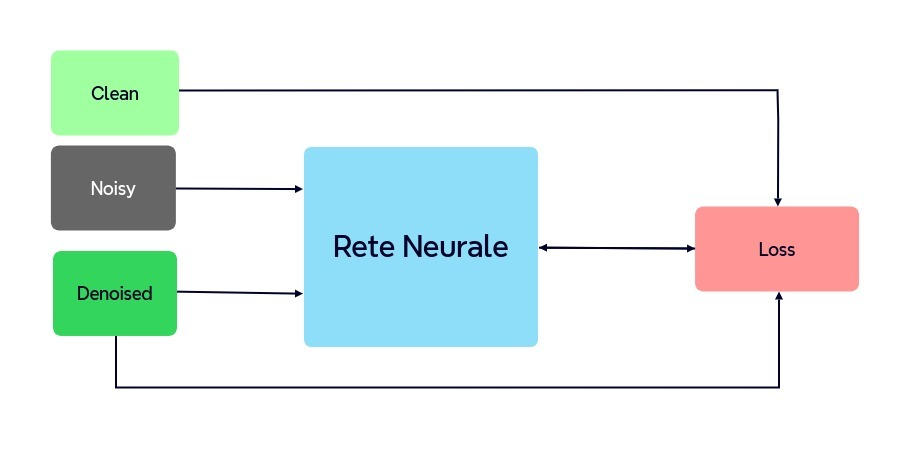
\includegraphics[width=0.8\textwidth]{utils/Architettura_rete_neurale.jpg}
    \caption{Mock della struttura logica per la previsione della qualità}
    \label{fig:MockReteNeurale}
\end{figure}

\section{Architettura rete neurale}
Come architettura della rete neurale è stata utilizzata la Unet. Questo perchè risulta particolarmente adatto per la 
generazione di una mappa di qualità che valuti l'affidabilità di un'immagine sottoposta a denoising. In letteratura si hanno articoli come 
Regional Image Quality Scoring for 2-D Echocardiography Using Deep Learning \cite{Vyver2025} che trattano dell'argomento. Il compito di 
questa rete è assegnare a ciascun pixel un valore compreso nell'intervallo $[0,1]$ che ne rappresenti la 
qualità locale. Questo output per la sua natura richiede un'architettura in grado di produrre una mappa di densità 
della stessa risoluzione spaziale dell'input, preservando la localizzazione precise delle informazioni. 
L'architettura trattata nell'articolo \textit{U-net: Convolutional networks for biomedical image segmentation} \cite{ronneberger2015unetconvolutionalnetworksbiomedical}, è composta da due parti principali: encoder e decoder. 
Encoder, ovvero una sequenza di blocchi convoluzionali e operazioni di pooling che estraggono feature 
gerarchiche via via più astratte, consentendo alla rete di catturare il contenuto semantico dell’immagine, 
distinguere texture, bordi e regioni omogenee, e modellare la natura statistica del rumore.
Decoder, una fase simmetrica che ricostruisce progressivamente la risoluzione spaziale 
mediante up-sampling e convoluzioni, trasformando le feature ad alto livello in una mappa di 
qualità densa e dettagliata.
Elemento distintivo della U-Net sono le skip connections, che collegano i livelli dell’encoder ai corrispondenti 
livelli del decoder. Questi collegamenti trasferiscono mappe di feature ad alta risoluzione direttamente al decoder, 
preservando l’informazione spaziale fine indispensabile per localizzare correttamente dettagli critici come bordi 
sottili e piccole texture. Senza tali connessioni, il decoder produrrebbe output più sfocati, perdendo la capacità 
di discriminare le aree più sensibili agli artefatti di oversmoothing o agli errori di ricostruzione.
L’aspetto più importante di questo modello è la sua capacità di andare oltre una semplice misura di errore pixel-wise. 
La rete apprende a sviluppare una vera e propria percezione semantica dell’errore, cioè a valutare la gravità di una 
discrepanza in funzione del contesto visivo in cui compare. Ad esempio, un errore di grande entità in una regione 
uniforme (come un cielo sereno) è visivamente più disturbante di un errore di pari entità in una regione altamente 
texturizzata (come del fogliame), dove può essere facilmente mascherato. Analogamente, un piccolo errore su un bordo 
netto è percettivamente rilevante. L’encoder, stratificando feature di complessità crescente, apprende questa gerarchia 
di contenuti visivi e fornisce al decoder le informazioni necessarie per produrre una mappa di qualità che pondera 
ogni errore in base alla sua importanza percettiva.

\section{Fusione dei modelli}
La fusione delle immagini denoised $[I]$ prodotte tramite i rispettivi modelli di despeckling vengono fusi attraverso una media pesata sfuttando
le mappa di qualità $[M]$ come pesi per le singole immagini.
\begin{equation}
    \makebox[\textwidth][c]{%
      $\displaystyle
        \frac{\sum_{i=1}^{n} I_i M_i}{\sum_{i=1}^{n} M_i}
      $%
    }
\end{equation}
Non è una fusione "cieca" (es. una media semplice). È un processo che si 
comporta in modo diverso per ogni singolo pixel dell'immagine. Se il Modello A ha una qualità stimata 
molto alta in una regione e il Modello B molto bassa, la fusione privilegerà maggiormente 
il Modello A in quella determinata area. Mentre alcuni sono eccellenti nel preservare i bordi netti ma possono lasciare del rumore residuo nelle aree lisce, 
altri sono ottimi nell' eliminare il rumore dalle superfici lisce ma tendono a sfocare (oversmooth) i bordi e le texture.
La fusione pesata permette di prendere il meglio di ogni modello usando di più l'output dell'algoritmo migliore per una data 
caratteristica dell'immagine, e meno i suoi contributi peggiori.
\\\\
\section{Funzione di loss}
Come funzione di perdità è stata utilizzata la mean square error [MSE] tra l'output della fusione [I] 
e il ground truth [$\hat{I}$], ovvero l'immagine clean . 
\begin{equation}
  \makebox[\textwidth][c]{%
    $\displaystyle
    \text{MSE} = \left( I - \hat{I} \right)^2
    $%
  }
\end{equation}
Questa funzione di perdità è stata scelta in quanto è molto facile da calcolare eccellenti 
non presenta particolari complicazioni in fase di ottimizzazzione. Inoltre 
dato che PSNR è funzione del MSE, ottimizzare la MSE porta anche ad avere valori 
più alti di PSNR, che spesso viene usato come metrica di valutazione 


\section{Metrica per la valutazione delle immagini despeckled}
Per la valutazione della qualità delle immagini despeckled è stata utilizzata la metrica PSNR come indicatore.
Il PSNR (Peak Signal-to-Noise Ratio) è una metrica usata per misurare la qualità di un’immagine ricostruita o 
compressa rispetto a un’immagine di riferimento (ground truth). 
Si basa sull’errore quadratico medio (MSE, Mean Squared Error) tra i pixel dell’immagine originale e 
quelli dell’immagine degradate/ricostruita. La formuala è: 
\begin{equation}
  \makebox[\textwidth][c]{%
    $\displaystyle
    \text{PSNR} = 10 \cdot \log_{10} \left( \frac{MAX_I^2}{\text{MSE}} \right)
    $%
  }
\end{equation}
Dove $MAX_I$ è il valore massimo possibile per un pixel. Più alto è il PSNR, migliore è la qualità dell’immagine ricostruita.

\section{Limiti dei questa tecnica}
Sebbene la media pesata presenti il vantaggio di combinare in maniera coerente i contributi dei vari modelli di despeckling, 
essa introduce alcune criticità che ne riducono l’efficacia in scenari complessi.
In primo luogo, la media pesata tende a diluire i dettagli sottili. Se una delle immagini denoised contiene strutture fini 
o bordi ben preservati che altre non hanno, questi dettagli possono risultare attenuati o addirittura persi, poiché la 
media li combina con le versioni più lisce prodotte dagli altri modelli. Ciò porta a un effetto di oversmoothing, che riduce 
il livello di dettaglio complessivo dell’immagine fusa.
Un’ulteriore limitazione deriva dal fatto che la media pesata opera pixel per pixel, senza considerare la correlazione spaziale 
tra pixel adiacenti. Pattern, texture e strutture complesse che sono distribuite su più pixel non vengono trattati in maniera 
coerente. Questo può portare a artefatti locali, soprattutto ai bordi o in aree con pattern ripetitivi, dove una decisione 
puramente puntuale può introdurre discontinuità.
Inoltre, se il rumore è altamente non stazionario o presenta componenti strutturate, la rete che genera le mappe di qualità 
può faticare a distinguere tra rumore residuo e dettaglio fine. In queste situazioni la mappa di qualità può risultare 
inaccurata, assegnando un peso elevato a regioni che in realtà presentano artefatti o penalizzando aree visivamente corrette. 
Questo porta a una fusione non ottimale, che può accentuare il rumore residuo o degradare regioni già ben restaurate.
Va considerato anche il problema della sensibilità agli errori di predizione della mappa di qualità. Poiché i pesi influenzano 
direttamente il risultato finale, eventuali errori nella stima della qualità si traducono in artefatti amplificati nell’immagine 
fusa, specialmente se un singolo modello viene sovrastimato in regioni dove la sua qualità non è affidabile.

% !TEX root = ../Thesis.tex

\subsection{Tabella di confronto tramite PSNR dei vari modelli}
\subsection{Tabella di confronto tramite PSNR dei vari modelli}
\begin{table}[H] % ambiente table per inserire una didascalia
  \centering
  \resizebox{1.3\textwidth}{!}{% <-- qui scegli quanto ridurla (0.9 = 90%)
    \begin{tabular}{|c|c|c|c|c|c|c|}
    \hline
    Bioma & SAR-CAM & FANS & SARBM3D & MEDIA & MEDIA PESATA & CrossFuse \\ \hline
    Agricultural &  24.95  & 24.58  & 25.37 & 18.92 & 19.07 & --- \\ \hline
    Airplane & 26.07 & 23.91 & 23.20 & 23.59 & 23.64 & --- \\ \hline
    Baseball diamond & 28.50 & 27.20 & 26.87 & 21.01 & 21.05 & --- \\ \hline
    Beach & 28.89 & 25.84 & 24.50 & 16.14 & 16.11 & --- \\ \hline
    Buldings & 24.51 & 22.23 & 21.52 & 21.93 & 21.89 & --- \\ \hline
    Chaparral & 22.93 & 21.49 & 22.43 & 18.57 & 18.78 & --- \\ \hline
    Forest & 26.48 & 25.66 & 25.97 & 17.81 & 18.44 & --- \\ \hline
    Freeway & 25.88 & 24.03 &  23.89 & 21.24 & 21.22 & --- \\ \hline
    Golf course& 28.41 & 27.23 & 26.97 & 20.79 & 20.86 & --- \\ \hline
    Harbor & 23.17 & 21.09 & 20.56 & 21.46 & 21.46 & --- \\ \hline
    intersection & 24.98 & 23.51 & 23.44 & 22.00 & 22.08 & --- \\ \hline
    mobile home park & 23.00 & 21.32 & 20.74 & 21.27 & 21.27 & --- \\ \hline
    Overpass & 25.46 & 23.79 & 23.56 & 23.19 & 23.19 & --- \\ \hline
    Parking lot & 22.36 & 21.01 & 20.69 & 21.24 & 21.24 & --- \\ \hline
    River & 25.76 & 24.86 & 25.03 & 19.72 & 19.72 & --- \\ \hline
    Runway & 27.22 & 24.88 & 24.82 & 20.51 & 20.51 & --- \\ \hline
    Sparse residential & 25.27 & 24.01 & 24.00 & 22.39 & 22.39 & --- \\ \hline
    Storage tanks & 25.67 & 23.63 & 22.91 & 22.12 & 22.12 & --- \\ \hline
    Tennis court & 25.99 & 24.70 & 24.62 & 21.77 & 21.77 & --- \\ \hline
    \end{tabular}
  } % fine resizebox
  \caption{Confronto dei modelli di despeckling e della loro fusione}
  \label{tab:esempio}
\end{table}


    I valori sopra, indicano la media del PSNR di 100 immagini rappresentanti diversi biomi.
    Ogni modello per la previsione della qualità, usato in TESI, 
    è stato allenato per 3 epoche con un dataset da 30'000 
    immagini. Come si puo notare dalla tabella [\ref{fig:MockReteNeurale}] 
    questa tecnica di fusione non valorizza al meglio i singoli modelli 
    portando il risultato finale ad essere peggiore di quello dei 
    singoli modelli presi singolarmente
    


